\begin{problem}{최장 경로}{standard input}{standard output}{1 second}{512 megabytes}

반지름이 $1$인 원 위에 $1$번부터 $N$번까지의 점이 시계 방향을 따라 동일한 간격으로 놓여 있다.

$1$번 점에서 출발하여 모든 점을 정확히 한 번씩 방문하려 한다. 단, 두 점 사이를 이동할 때는 두 점을 잇는 선분을 따라 이동해야 한다. 이러한 경로 중 길이가 가장 긴 경로를 구하여라.

\InputFile
첫 줄에 $N(2 \le N \le 2\cdot10^5)$이 주어진다.

\OutputFile
길이가 가장 긴 경로에 대해 지나가는 점의 번호를 공백으로 구분하여 순서대로 출력하여라. 만약 그러한 경로가 여러 개라면 아무거나 하나를 출력한다.

\Examples

\begin{example}
\exmpfile{files/example.01}{files/example.01.a}%
\exmpfile{files/example.02}{files/example.02.a}%
\end{example}

\Note
두 번째 예제에서 경로를 그림으로 나타내면 아래와 같다. 경로의 길이는 $4+\sqrt{2}$로 이보다 긴 경로는 존재하지 않는다.

\begin{center}
    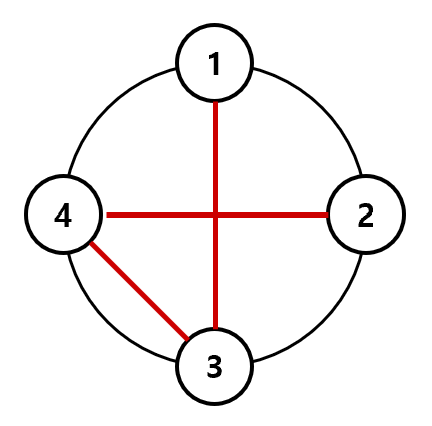
\includegraphics[width=4cm]{files/longest_path_ex.png}
\end{center}

\end{problem}

